\chapter{Introduction}\label{cha:intro}

Data processing is required by every modern business in some form. Existing solutions like SQL fit the requirements of the majority of use cases, as the volume of data they process can be contained within a single system. However, as the volumes of data begin to increase, in particular over around 100GB of raw data, single system solutions like SQL begin to struggle as not all of the data can be loaded into memory at once. 

Figure \ref{fig:single-system-solution} shows the network model when using a single system to perform data processing on a SQL server. A number of clients are all connected to a single server, and the server can become overloaded if a large number of clients are making intensive queries, or if some of the queries operate on a large amount of data. This results in significantly reduced query performance, or even outright failure, because the system must spend a large amount of time moving data in and out of memory to perform the computation. It is possible to make extremely powerful servers, but ultimately these solutions are constrained to a single machine, meaning there is an upper limit to the compute performance based on the current technology available.

\begin{figure}[h]
	\centering
	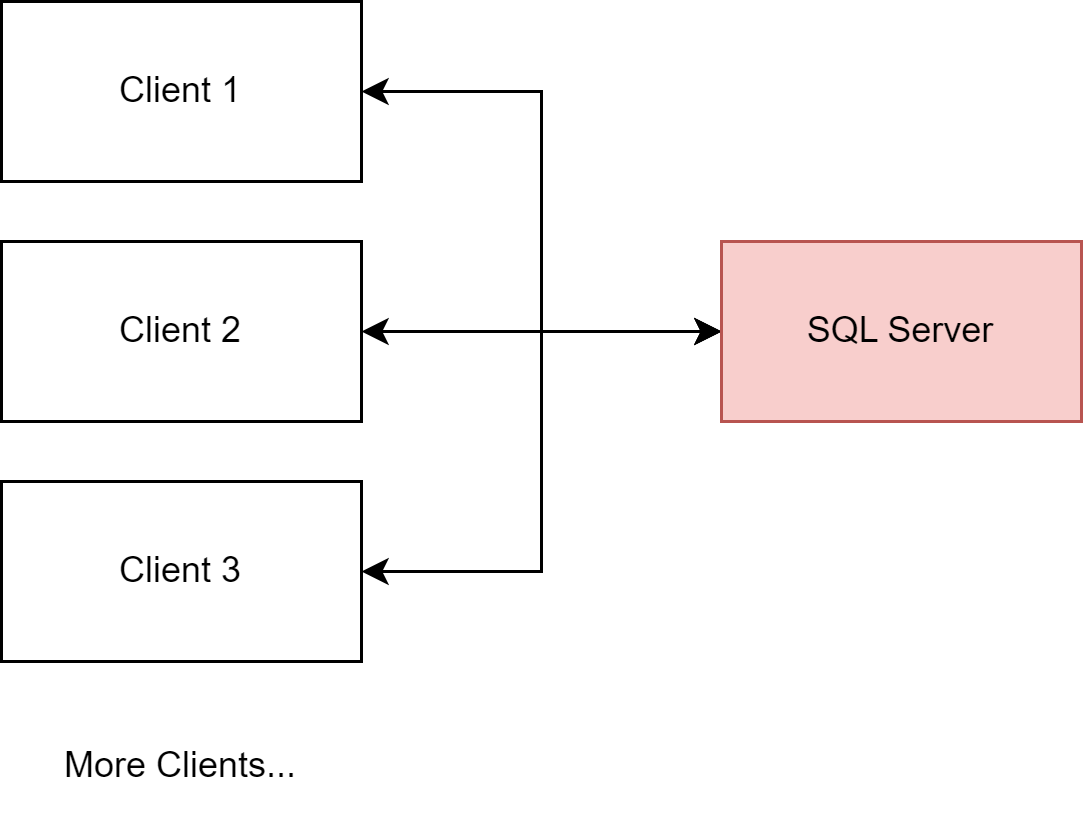
\includegraphics[width=0.4\textwidth]{chapters/diagrams/design/single-system-solution}
	\caption{Single System Solution}
	\label{fig:single-system-solution}
\end{figure}

This type of processing is generally used in \textit{extract-transform-load} (ETL) workflows, which describe the type of workflow where data must be imported in bulk from some external source, processed in some relatively simple way, then exported elsewhere for further analysis. Often, the processing to be performed acts on small groups of rows in the original dataset at once. This is usually a unit item within the dataset, for example a loan, customer, or product. As a result, even if the overall dataset is extremely large, the processing can be easily parallelised, as only a small number of rows are needed at any one time to produce the required output.

Distributed systems therefore present an excellent opportunity for solving this problem. If a system can be designed to automatically split a dataset up and perform the processing over a number of nodes in a cluster, this system could potentially be able to process data of any size; larger datasets can be accommodated by simply increasing the number of nodes in the cluster. Similarly, to an extent a query can always be processed faster by increasing the number of nodes, or the performance of each node.

% Why is this area important, why am I investigating it
% More general big data references here - difficulties faced due to larger than memory data sets
% References to ETL if possible, and how this is an increasingly important workflow.

\section{Prior Work}
Distributed Data Processing has existed conceptually since as early as the 1970s. A key paper by Philip Enslow Jr{\frenchspacing.} from this period sets out characteristics across three 'dimensions' of decentralisation: hardware (the number of machines involved in the computation), control (the management of the cluster), and database (decentralisation of storage) \cite{enslow1978distributed}. Enslow argued that these dimensions defined a distributed system, while also acknowledging that the technology of the period was not equipped to fulfil the goals he laid out.

Research into solutions for distributed data processing has generally resulted in two kinds of solutions \cite{yaqoob2016big}:
\begin{itemize}
	\item \textbf{Batch processing:} where data is gathered, processed and output all at the same time. This includes solutions like MapReduce and Spark  \cite{dean2008mapreduce, zaharia2016spark}. Batch processing works best for data that can be considered 'complete' at some stage.
	\item \textbf{Stream processing:} where data is processed and output as it arrives. This includes solutions like Apache Flink, Storm, and Spark Streaming \cite{carbone2015flink, toshniwal2014storm, armbrust2018sparkstreaming}. Stream processing works best for data that is being constantly generated, and needs to be analysed as it arrives.
\end{itemize}

MapReduce, a framework introduced by Google in the mid 2000s, could be considered the breakthrough framework for performing massively scalable, parallelised data processing \cite{dean2008mapreduce}. This framework later became one of the core modules for the Apache Hadoop suite of tools. It provided a simple API, where developers could describe a job as a \textit{map} and a \textit{reduce} step, and the framework would handle the specifics of managing the distributed system. 

While MapReduce was Google's offering, other large technology companies had similar solutions, including Microsoft, who created DryadLINQ in 2009 \cite{fetterly2009dryadlinq}. However, due to the massive success of MapReduce, Microsoft discontinued DryadLINQ in 2011.

MapReduce was not without flaws, and many papers were published in the years following its initial release which performed performance benchmarks, and analysed its strengths and weaknesses \cite{lee2012parallel}. Crucially, MapReduce appears to particularly struggle with iterative algorithms which are performed over a number of steps, as it relies on reading and writing to a persistent storage format after each step. A number of popular extensions to MapReduce were introduced to improve the performance on iterative algorithms, like Twister and HaLoop both in 2010 \cite{ekanayake2010twister, bu2010haloop}.

MapReduce was challenging to use for developers used to more traditional data processing tools like SQL due to its imperative programming style, resulting in a number of tools being created to improve its usability and accessibility. Hive is one such tool, which features a SQL-like language called HiveQL to allow users to write declarative programs that compiled into MapReduce jobs \cite{thusoo2010hive}. Pig Latin is similar, and features a mixed declarative and imperative language style that again compiles down into MapReduce jobs \cite{olston2008pig}. Further tools in the wider areas of the field were introduced around 2010, including another project by Google named Pregel, specialised for performing distributed data processing on large-scale graphs \cite{malewicz2010pregel}.

% Spark - initial creation, talk specifically about RDDs
In 2010, the first paper on Spark was released \cite{zaharia2010spark}. Spark aims to improve upon MapReduce's weaknesses, by storing data in memory and providing fault tolerance by tracking the 'lineage' of data. This means for any set of data, Spark knows how the data was constructed from another persistent, fault tolerant data source, and can use that to reconstruct any lost data in the event of failure. This in-memory storage, known as a resilient distributed dataset (RDD) allows Spark to improve on MapReduce's performance for iterative jobs, whilst also allowing it to quickly perform ad-hoc queries \cite{zaharia2012rdd}. Effectively, Spark is strong at performing long batch jobs, as well as short interactive queries. This approach was successful at resolving MapReduce's weakness for iterative algorithms, as keeping the data in-memory removes the read-write overhead that caused MapReduce's performance problems. 

% Spark - extensions - SQL, Streaming
Spark quickly grew in popularity, with a number of extensions being added to improve its usability, including a SQL-style engine with a query optimiser, as well as an engine supporting stream processing \cite{armbrust2015sparksql, armbrust2018sparkstreaming}. A second paper released in 2016 stated that Spark was in use in thousands of organisations, with the largest deployment running an 8,000 node cluster holding 100PB of data \cite{zaharia2016spark}. Spark is designed to be agnostic of any particular storage mechanism. Instead, it relies on custom connectors to retrieve data from various sources. This provides the advantage that Spark can interface with a large number of data sources, but it is not specialised at retrieving source data from any of them, presenting an opportunity for a new solution to improve on data import speed through close integration with the persistent storage mechanism.

% Stream processing tools - not entirely what I'm looking at, but still within the field - Kafka, Storm
More recent research indicates that the future of the field is moving away from batch processing, and towards stream processing for data that is constantly being generated. A 2015 paper by Google argues that the volumes of data, the fact that datasets can no longer ever be considered 'complete', along with demands for improved insight into the data means that streaming 'dataflow' models are the way forward  \cite{akidau2015dataflow}. Google publicly stated in their 2014 'Google I/O' Keynote that they were phasing out MapReduce in their internal systems \cite{googleio2014}. The input data for the system is expected to be imported in bulk, and is not being received at a constant rate. As such, designing for a streaming solution is not required in this case.

\section{Project Aims} \todo{vincent intro suggestions}
The objective of this project is to design a query processing engine to perform data processing over a distributed cluster of nodes. To ensure maximum accessibility for users of existing data processing tools, the system should feature a SQL-like interface implemented in a widely-used language. This will allow it to be used for ETL workflows, where large data volumes often cause problems. Finally, as this will be designed as an all-in-one solution, the system should attempt to exploit the integration between the storage mechanism and nodes performing the computation to improve the execution speed; this appears to be an area where existing distributed data processing solutions struggle to perform as effectively.

% Reiterate high level aim, explain how my solution will differ from prior work discussed
% Focus on grouped data, and improving access efficiency for that
% Easy-to-use Python interface

